% Options for packages loaded elsewhere
\PassOptionsToPackage{unicode}{hyperref}
\PassOptionsToPackage{hyphens}{url}
\PassOptionsToPackage{dvipsnames,svgnames,x11names}{xcolor}
%
\documentclass[
  letterpaper,
  DIV=11,
  numbers=noendperiod]{scrartcl}

\usepackage{amsmath,amssymb}
\usepackage{iftex}
\ifPDFTeX
  \usepackage[T1]{fontenc}
  \usepackage[utf8]{inputenc}
  \usepackage{textcomp} % provide euro and other symbols
\else % if luatex or xetex
  \usepackage{unicode-math}
  \defaultfontfeatures{Scale=MatchLowercase}
  \defaultfontfeatures[\rmfamily]{Ligatures=TeX,Scale=1}
\fi
\usepackage{lmodern}
\ifPDFTeX\else  
    % xetex/luatex font selection
\fi
% Use upquote if available, for straight quotes in verbatim environments
\IfFileExists{upquote.sty}{\usepackage{upquote}}{}
\IfFileExists{microtype.sty}{% use microtype if available
  \usepackage[]{microtype}
  \UseMicrotypeSet[protrusion]{basicmath} % disable protrusion for tt fonts
}{}
\makeatletter
\@ifundefined{KOMAClassName}{% if non-KOMA class
  \IfFileExists{parskip.sty}{%
    \usepackage{parskip}
  }{% else
    \setlength{\parindent}{0pt}
    \setlength{\parskip}{6pt plus 2pt minus 1pt}}
}{% if KOMA class
  \KOMAoptions{parskip=half}}
\makeatother
\usepackage{xcolor}
\setlength{\emergencystretch}{3em} % prevent overfull lines
\setcounter{secnumdepth}{5}
% Make \paragraph and \subparagraph free-standing
\makeatletter
\ifx\paragraph\undefined\else
  \let\oldparagraph\paragraph
  \renewcommand{\paragraph}{
    \@ifstar
      \xxxParagraphStar
      \xxxParagraphNoStar
  }
  \newcommand{\xxxParagraphStar}[1]{\oldparagraph*{#1}\mbox{}}
  \newcommand{\xxxParagraphNoStar}[1]{\oldparagraph{#1}\mbox{}}
\fi
\ifx\subparagraph\undefined\else
  \let\oldsubparagraph\subparagraph
  \renewcommand{\subparagraph}{
    \@ifstar
      \xxxSubParagraphStar
      \xxxSubParagraphNoStar
  }
  \newcommand{\xxxSubParagraphStar}[1]{\oldsubparagraph*{#1}\mbox{}}
  \newcommand{\xxxSubParagraphNoStar}[1]{\oldsubparagraph{#1}\mbox{}}
\fi
\makeatother

\usepackage{color}
\usepackage{fancyvrb}
\newcommand{\VerbBar}{|}
\newcommand{\VERB}{\Verb[commandchars=\\\{\}]}
\DefineVerbatimEnvironment{Highlighting}{Verbatim}{commandchars=\\\{\}}
% Add ',fontsize=\small' for more characters per line
\usepackage{framed}
\definecolor{shadecolor}{RGB}{241,243,245}
\newenvironment{Shaded}{\begin{snugshade}}{\end{snugshade}}
\newcommand{\AlertTok}[1]{\textcolor[rgb]{0.68,0.00,0.00}{#1}}
\newcommand{\AnnotationTok}[1]{\textcolor[rgb]{0.37,0.37,0.37}{#1}}
\newcommand{\AttributeTok}[1]{\textcolor[rgb]{0.40,0.45,0.13}{#1}}
\newcommand{\BaseNTok}[1]{\textcolor[rgb]{0.68,0.00,0.00}{#1}}
\newcommand{\BuiltInTok}[1]{\textcolor[rgb]{0.00,0.23,0.31}{#1}}
\newcommand{\CharTok}[1]{\textcolor[rgb]{0.13,0.47,0.30}{#1}}
\newcommand{\CommentTok}[1]{\textcolor[rgb]{0.37,0.37,0.37}{#1}}
\newcommand{\CommentVarTok}[1]{\textcolor[rgb]{0.37,0.37,0.37}{\textit{#1}}}
\newcommand{\ConstantTok}[1]{\textcolor[rgb]{0.56,0.35,0.01}{#1}}
\newcommand{\ControlFlowTok}[1]{\textcolor[rgb]{0.00,0.23,0.31}{\textbf{#1}}}
\newcommand{\DataTypeTok}[1]{\textcolor[rgb]{0.68,0.00,0.00}{#1}}
\newcommand{\DecValTok}[1]{\textcolor[rgb]{0.68,0.00,0.00}{#1}}
\newcommand{\DocumentationTok}[1]{\textcolor[rgb]{0.37,0.37,0.37}{\textit{#1}}}
\newcommand{\ErrorTok}[1]{\textcolor[rgb]{0.68,0.00,0.00}{#1}}
\newcommand{\ExtensionTok}[1]{\textcolor[rgb]{0.00,0.23,0.31}{#1}}
\newcommand{\FloatTok}[1]{\textcolor[rgb]{0.68,0.00,0.00}{#1}}
\newcommand{\FunctionTok}[1]{\textcolor[rgb]{0.28,0.35,0.67}{#1}}
\newcommand{\ImportTok}[1]{\textcolor[rgb]{0.00,0.46,0.62}{#1}}
\newcommand{\InformationTok}[1]{\textcolor[rgb]{0.37,0.37,0.37}{#1}}
\newcommand{\KeywordTok}[1]{\textcolor[rgb]{0.00,0.23,0.31}{\textbf{#1}}}
\newcommand{\NormalTok}[1]{\textcolor[rgb]{0.00,0.23,0.31}{#1}}
\newcommand{\OperatorTok}[1]{\textcolor[rgb]{0.37,0.37,0.37}{#1}}
\newcommand{\OtherTok}[1]{\textcolor[rgb]{0.00,0.23,0.31}{#1}}
\newcommand{\PreprocessorTok}[1]{\textcolor[rgb]{0.68,0.00,0.00}{#1}}
\newcommand{\RegionMarkerTok}[1]{\textcolor[rgb]{0.00,0.23,0.31}{#1}}
\newcommand{\SpecialCharTok}[1]{\textcolor[rgb]{0.37,0.37,0.37}{#1}}
\newcommand{\SpecialStringTok}[1]{\textcolor[rgb]{0.13,0.47,0.30}{#1}}
\newcommand{\StringTok}[1]{\textcolor[rgb]{0.13,0.47,0.30}{#1}}
\newcommand{\VariableTok}[1]{\textcolor[rgb]{0.07,0.07,0.07}{#1}}
\newcommand{\VerbatimStringTok}[1]{\textcolor[rgb]{0.13,0.47,0.30}{#1}}
\newcommand{\WarningTok}[1]{\textcolor[rgb]{0.37,0.37,0.37}{\textit{#1}}}

\providecommand{\tightlist}{%
  \setlength{\itemsep}{0pt}\setlength{\parskip}{0pt}}\usepackage{longtable,booktabs,array}
\usepackage{calc} % for calculating minipage widths
% Correct order of tables after \paragraph or \subparagraph
\usepackage{etoolbox}
\makeatletter
\patchcmd\longtable{\par}{\if@noskipsec\mbox{}\fi\par}{}{}
\makeatother
% Allow footnotes in longtable head/foot
\IfFileExists{footnotehyper.sty}{\usepackage{footnotehyper}}{\usepackage{footnote}}
\makesavenoteenv{longtable}
\usepackage{graphicx}
\makeatletter
\newsavebox\pandoc@box
\newcommand*\pandocbounded[1]{% scales image to fit in text height/width
  \sbox\pandoc@box{#1}%
  \Gscale@div\@tempa{\textheight}{\dimexpr\ht\pandoc@box+\dp\pandoc@box\relax}%
  \Gscale@div\@tempb{\linewidth}{\wd\pandoc@box}%
  \ifdim\@tempb\p@<\@tempa\p@\let\@tempa\@tempb\fi% select the smaller of both
  \ifdim\@tempa\p@<\p@\scalebox{\@tempa}{\usebox\pandoc@box}%
  \else\usebox{\pandoc@box}%
  \fi%
}
% Set default figure placement to htbp
\def\fps@figure{htbp}
\makeatother

% load packages
\usepackage{geometry}
\usepackage{xcolor}
\usepackage{eso-pic}
\usepackage{fancyhdr}
\usepackage{sectsty}
\usepackage{fontspec}
\usepackage{titlesec}

%% Set page size with a wider right margin
\geometry{a4paper, total={170mm,257mm}, left=20mm, top=20mm, bottom=20mm, right=50mm}

%% Let's define some colours
\definecolor{light}{HTML}{E6E6FA}
\definecolor{highlight}{HTML}{800080}
\definecolor{dark}{HTML}{330033}

%% Let's add the border on the right hand side 
\AddToShipoutPicture{% 
    \AtPageLowerLeft{% 
        \put(\LenToUnit{\dimexpr\paperwidth-3cm},0){% 
            \color{light}\rule{3cm}{\LenToUnit\paperheight}%
          }%
     }%
     % logo
    \AtPageLowerLeft{% start the bar at the bottom right of the page
        \put(\LenToUnit{\dimexpr\paperwidth-2.25cm},27.2cm){% move it to the top right
            \color{light}
\includegraphics[width=1.5cm]{_extensions/nrennie/PrettyPDF/logo.png}
          }%
     }%
}

%% Style the page number
\fancypagestyle{mystyle}{
  \fancyhf{}
  \renewcommand\headrulewidth{0pt}
  \fancyfoot[R]{\thepage}
  \fancyfootoffset{3.5cm}
}
\setlength{\footskip}{20pt}

%% style the chapter/section fonts
\chapterfont{\color{dark}\fontsize{20}{16.8}\selectfont}
\sectionfont{\color{dark}\fontsize{20}{16.8}\selectfont}
\subsectionfont{\color{dark}\fontsize{14}{16.8}\selectfont}
\titleformat{\subsection}
  {\sffamily\Large\bfseries}{\thesection}{1em}{}[{\titlerule[0.8pt]}]
  
% left align title
\makeatletter
\renewcommand{\maketitle}{\bgroup\setlength{\parindent}{0pt}
\begin{flushleft}
  {\sffamily\huge\textbf{\MakeUppercase{\@title}}} \vspace{0.3cm} \newline
  {\Large {\@subtitle}} \newline
  \@author
\end{flushleft}\egroup
}
\makeatother

%% Use some custom fonts
\setsansfont{Ubuntu}[
    Path=_extensions/nrennie/PrettyPDF/Ubuntu/,
    Scale=0.9,
    Extension = .ttf,
    UprightFont=*-Regular,
    BoldFont=*-Bold,
    ItalicFont=*-Italic,
    ]

\setmainfont{Ubuntu}[
    Path=_extensions/nrennie/PrettyPDF/Ubuntu/,
    Scale=0.9,
    Extension = .ttf,
    UprightFont=*-Regular,
    BoldFont=*-Bold,
    ItalicFont=*-Italic,
    ]
\KOMAoption{captions}{tableheading}
\makeatletter
\@ifpackageloaded{tcolorbox}{}{\usepackage[skins,breakable]{tcolorbox}}
\@ifpackageloaded{fontawesome5}{}{\usepackage{fontawesome5}}
\definecolor{quarto-callout-color}{HTML}{909090}
\definecolor{quarto-callout-note-color}{HTML}{0758E5}
\definecolor{quarto-callout-important-color}{HTML}{CC1914}
\definecolor{quarto-callout-warning-color}{HTML}{EB9113}
\definecolor{quarto-callout-tip-color}{HTML}{00A047}
\definecolor{quarto-callout-caution-color}{HTML}{FC5300}
\definecolor{quarto-callout-color-frame}{HTML}{acacac}
\definecolor{quarto-callout-note-color-frame}{HTML}{4582ec}
\definecolor{quarto-callout-important-color-frame}{HTML}{d9534f}
\definecolor{quarto-callout-warning-color-frame}{HTML}{f0ad4e}
\definecolor{quarto-callout-tip-color-frame}{HTML}{02b875}
\definecolor{quarto-callout-caution-color-frame}{HTML}{fd7e14}
\makeatother
\makeatletter
\@ifpackageloaded{caption}{}{\usepackage{caption}}
\AtBeginDocument{%
\ifdefined\contentsname
  \renewcommand*\contentsname{Table of contents}
\else
  \newcommand\contentsname{Table of contents}
\fi
\ifdefined\listfigurename
  \renewcommand*\listfigurename{List of Figures}
\else
  \newcommand\listfigurename{List of Figures}
\fi
\ifdefined\listtablename
  \renewcommand*\listtablename{List of Tables}
\else
  \newcommand\listtablename{List of Tables}
\fi
\ifdefined\figurename
  \renewcommand*\figurename{Figure}
\else
  \newcommand\figurename{Figure}
\fi
\ifdefined\tablename
  \renewcommand*\tablename{Table}
\else
  \newcommand\tablename{Table}
\fi
}
\@ifpackageloaded{float}{}{\usepackage{float}}
\floatstyle{ruled}
\@ifundefined{c@chapter}{\newfloat{codelisting}{h}{lop}}{\newfloat{codelisting}{h}{lop}[chapter]}
\floatname{codelisting}{Listing}
\newcommand*\listoflistings{\listof{codelisting}{List of Listings}}
\makeatother
\makeatletter
\makeatother
\makeatletter
\@ifpackageloaded{caption}{}{\usepackage{caption}}
\@ifpackageloaded{subcaption}{}{\usepackage{subcaption}}
\makeatother
\makeatletter
\@ifpackageloaded{tcolorbox}{}{\usepackage[skins,breakable]{tcolorbox}}
\makeatother
\makeatletter
\@ifundefined{shadecolor}{\definecolor{shadecolor}{rgb}{.97, .97, .97}}{}
\makeatother
\makeatletter
\@ifundefined{codebgcolor}{\definecolor{codebgcolor}{named}{light}}{}
\makeatother
\makeatletter
\ifdefined\Shaded\renewenvironment{Shaded}{\begin{tcolorbox}[sharp corners, colback={codebgcolor}, frame hidden, enhanced, boxrule=0pt, breakable]}{\end{tcolorbox}}\fi
\makeatother

\usepackage{bookmark}

\IfFileExists{xurl.sty}{\usepackage{xurl}}{} % add URL line breaks if available
\urlstyle{same} % disable monospaced font for URLs
\hypersetup{
  pdftitle={Practical 4},
  colorlinks=true,
  linkcolor={highlight},
  filecolor={Maroon},
  citecolor={Blue},
  urlcolor={highlight},
  pdfcreator={LaTeX via pandoc}}


\title{Practical 4}
\author{}
\date{}

\begin{document}
\maketitle

\pagestyle{mystyle}


\textbf{Aim of this practical:}

\begin{enumerate}
\def\labelenumi{\arabic{enumi}.}
\tightlist
\item
  Work with different types of spatial data types including: Areal,
  Geostatistical and Spatial Point process data.
\item
  Read and visualize shapefiles into R
\item
  Manipulate and visualize \texttt{sf} spatial object in R
\item
  Manipulate and visualize raster data in R.
\end{enumerate}

we are going to learn:

\begin{itemize}
\tightlist
\item
  Explore tools for spatial data wrangling and visualization.
\item
  Use some commonly used metrics to assess spatial autocorrelation in
  our data.
\end{itemize}

In this practical we will:

\begin{itemize}
\tightlist
\item
  Explore tools for areal spatial data wrangling and visualization.
\item
  Compute Morans'I to identify spatial autocorrelation in our data.
\end{itemize}

\subsection{Areal (lattice) data}\label{sec-areal_data}

Areal data our measurements are summarised across a set of discrete,
non-overlapping spatial units such as postcode areas, health board or
pixels on a satellite image. In consequence, the spatial domain is a
countable collection of (regular or irregular) areal units at which
variables are observed. Many public health studies use data aggregated
over groups rather than data on individuals - often this is for privacy
reasons, but it may also be for convenience.

In the next example we are going to explore data on respiratory
hospitalisations for Greater Glasgow and Clyde between 2007 and 2011.
The data are available from the \texttt{CARBayesdata} R Package:

\begin{Shaded}
\begin{Highlighting}[]
\FunctionTok{library}\NormalTok{(CARBayesdata)}

\FunctionTok{data}\NormalTok{(pollutionhealthdata)}
\FunctionTok{data}\NormalTok{(GGHB.IZ)}
\end{Highlighting}
\end{Shaded}

The \texttt{pollutionhealthdata} contains the spatiotemporal data on
respiratory hospitalisations, air pollution concentrations and
socio-economic deprivation covariates for the 271 Intermediate Zones
(IZ) that make up the Greater Glasgow and Clyde health board in
Scotland. Data are provided by the
\href{http://statistics.gov.scot.}{Scottish Government} and the
available variables are:

\begin{itemize}
\tightlist
\item
  \texttt{IZ}: unique identifier for each IZ.
\item
  \texttt{year}: the year were the measruments were taken
\item
  \texttt{observed}: observed numbers of hospitalisations due to
  respiratory disease.
\item
  \texttt{expected}: expected numbers of hospitalisations due to
  respiratory disease computed using indirect standardisation from
  Scotland-wide respiratory hospitalisation rates.
\item
  \texttt{pm10}: Average particulate matter (less than 10 microns)
  concentrations.
\item
  \texttt{jsa}: The percentage of working age people who are in receipt
  of Job Seekers Allowance
\item
  \texttt{price}: Average property price (divided by 100,000).
\end{itemize}

The \texttt{GGHB.IZ} data is a Simple Features (\texttt{sf}) object
containing the spatial polygon information for the set of 271
Intermediate Zones (IZ), that make up of the Greater Glasgow and Clyde
health board in Scotland ( Figure~\ref{fig-GGC} ).

\begin{figure}

\centering{

\pandocbounded{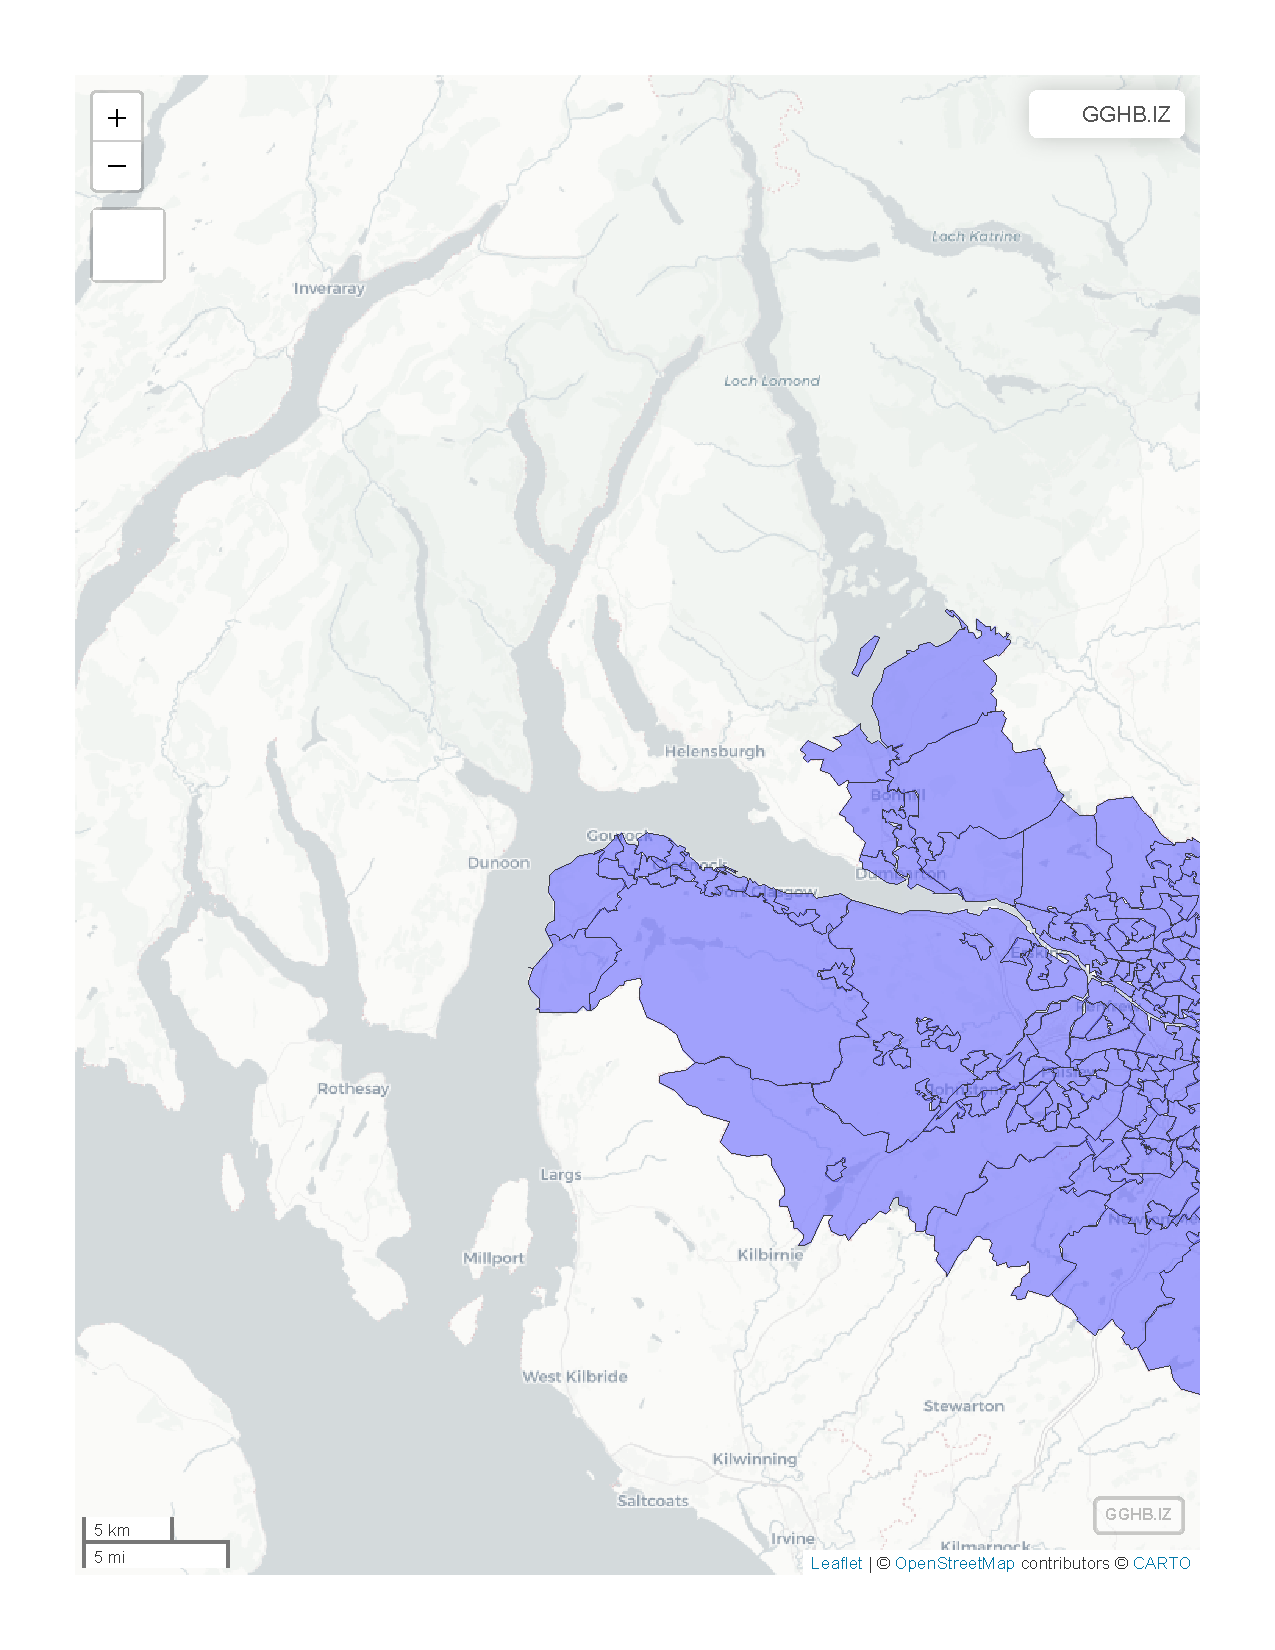
\includegraphics[keepaspectratio]{day2_practical_4_files/figure-pdf/fig-GGC-1.pdf}}

}

\caption{\label{fig-GGC}Greater Glasgow and Clyde health board
represented by 271 Intermediate Zones}

\end{figure}%

Let's start by loading useful libraries:

\begin{Shaded}
\begin{Highlighting}[]
\FunctionTok{library}\NormalTok{(sf)}
\FunctionTok{library}\NormalTok{(ggplot2)}
\FunctionTok{library}\NormalTok{(scico)}
\end{Highlighting}
\end{Shaded}

The \texttt{sf} package allows us to work with vector data which is used
to represent points, lines, and polygons. It can also be used to read
vector data stored as a shapefiles.

First, lets combine both data sets based on the Intermediate Zones (IZ)
variable using the \texttt{merge} function from \texttt{base} R:

\begin{Shaded}
\begin{Highlighting}[]
\NormalTok{resp\_cases }\OtherTok{\textless{}{-}} \FunctionTok{merge}\NormalTok{(GGHB.IZ, pollutionhealthdata, }\AttributeTok{by =} \StringTok{"IZ"}\NormalTok{)}
\end{Highlighting}
\end{Shaded}

In epidemiology, disease risk is usually estimated using Standardized
Mortality Ratios (SMR). The SMR for a given spatial areal unit \(i\) is
defined as the ratio between the observed ( \(Y_i\) ) and expected (
\(E_i\) ) number of cases:

\[
SMR_i = \dfrac{Y_i}{E_i}
\]

A value \(SMR > 1\) indicates that there are more observed cases than
expected which corresponds to a high risk area. On the other hand, if
\(SMR<1\) then there are fewer observed cases than expected, suggesting
a low risk area.

We can manipulate \texttt{sf} objects the same way we manipulate
standard data frame objects via the \texttt{dplyr} package. Lets use the
pipeline command \texttt{\%\textgreater{}\%} and the \texttt{mutate}
function to calculate the yearly SMR values for each IZ:

\begin{Shaded}
\begin{Highlighting}[]
\FunctionTok{library}\NormalTok{(dplyr)}
\NormalTok{resp\_cases }\OtherTok{\textless{}{-}}\NormalTok{ resp\_cases }\SpecialCharTok{\%\textgreater{}\%} 
  \FunctionTok{mutate}\NormalTok{(}\AttributeTok{SMR =}\NormalTok{ observed}\SpecialCharTok{/}\NormalTok{expected, }\AttributeTok{.by =}\NormalTok{ year )}
\end{Highlighting}
\end{Shaded}

Now we use \texttt{ggplot} to visualize our data by adding a
\texttt{geom\_sf} layer and coloring it according to our variable of
interest (i.e., SMR). We can further use \texttt{facet\_wrap} to create
a layer per year and chose an appropriate color palette using the
\texttt{scale\_fill\_scico} from the \texttt{scico} package:

\begin{Shaded}
\begin{Highlighting}[]
\FunctionTok{ggplot}\NormalTok{()}\SpecialCharTok{+}
  \FunctionTok{geom\_sf}\NormalTok{(}\AttributeTok{data=}\NormalTok{resp\_cases,}\FunctionTok{aes}\NormalTok{(}\AttributeTok{fill=}\NormalTok{SMR))}\SpecialCharTok{+}
  \FunctionTok{facet\_wrap}\NormalTok{(}\SpecialCharTok{\textasciitilde{}}\NormalTok{year)}\SpecialCharTok{+}\FunctionTok{scale\_fill\_scico}\NormalTok{(}\AttributeTok{palette =} \StringTok{"roma"}\NormalTok{)}
\end{Highlighting}
\end{Shaded}

\begin{center}
\pandocbounded{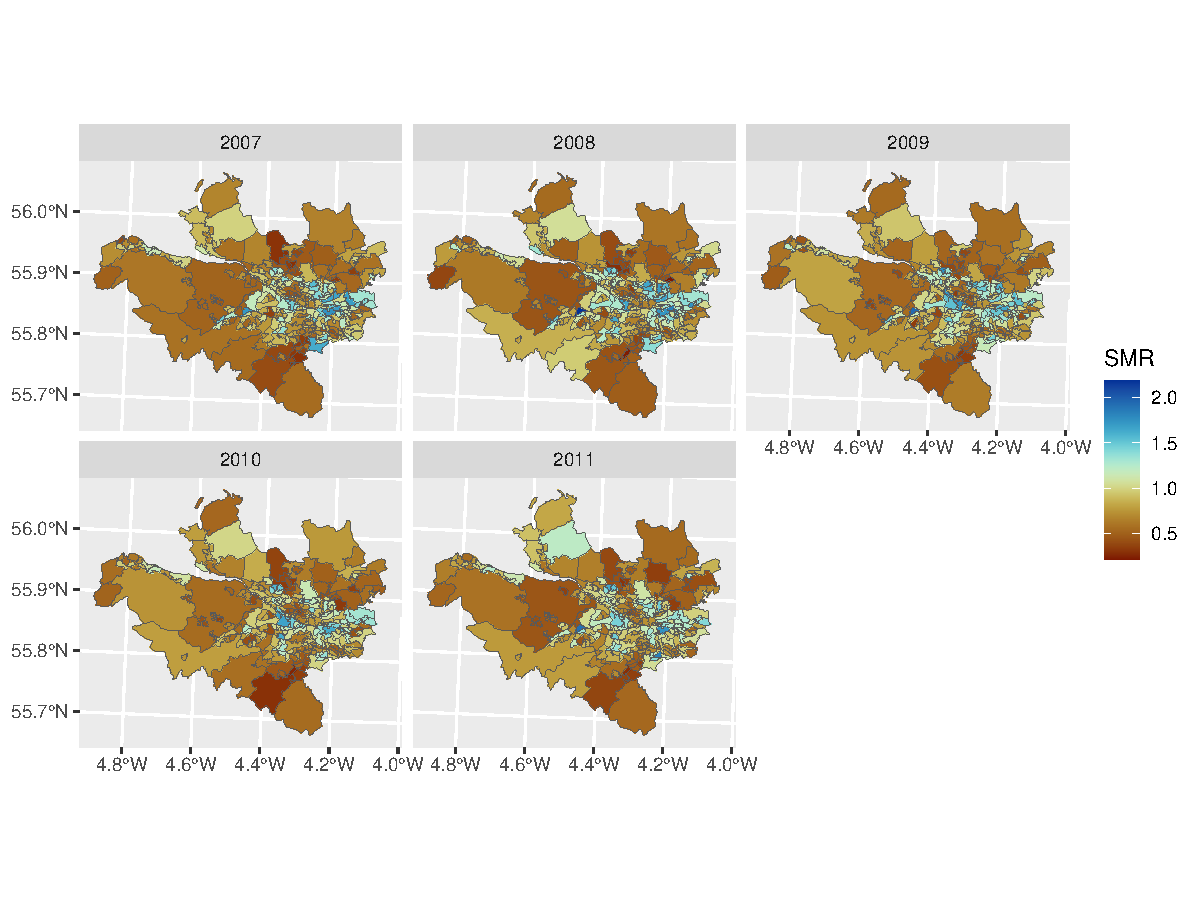
\includegraphics[keepaspectratio]{day2_practical_4_files/figure-pdf/unnamed-chunk-11-1.pdf}}
\end{center}

\begin{tcolorbox}[enhanced jigsaw, bottomrule=.15mm, toprule=.15mm, rightrule=.15mm, arc=.35mm, coltitle=black, leftrule=.75mm, colframe=quarto-callout-warning-color-frame, colback=white, left=2mm, colbacktitle=quarto-callout-warning-color!10!white, bottomtitle=1mm, toptitle=1mm, titlerule=0mm, title={Task}, opacitybacktitle=0.6, opacityback=0, breakable]

Produce a map that shows the spatial distribution of each of the
following variables for the year 2011:

\begin{itemize}
\item
  Average particulate matter \texttt{pm10}
\item
  Average property price \texttt{price}
\item
  Percentage of working age people who are in receipt of Job Seekers
  Allowance \texttt{jsa}
\end{itemize}

hint

You can use the \texttt{filter} function from \texttt{dplyr} to subset
the data according to the year of interest.

Click here to see the solution

\begin{Shaded}
\begin{Highlighting}[]
\CommentTok{\# Library for plotting multiple maps together}

\FunctionTok{library}\NormalTok{(patchwork)}

\CommentTok{\# subset data set for 2011}

\NormalTok{resp\_cases\_2011 }\OtherTok{\textless{}{-}}\NormalTok{ resp\_cases }\SpecialCharTok{\%\textgreater{}\%} \FunctionTok{filter}\NormalTok{(year }\SpecialCharTok{==}\DecValTok{2011}\NormalTok{)}

\CommentTok{\# pm10 plot}

\NormalTok{pm10\_plot }\OtherTok{\textless{}{-}} \FunctionTok{ggplot}\NormalTok{()}\SpecialCharTok{+}
  \FunctionTok{geom\_sf}\NormalTok{(}\AttributeTok{data=}\NormalTok{resp\_cases\_2011,}\FunctionTok{aes}\NormalTok{(}\AttributeTok{fill=}\NormalTok{pm10))}\SpecialCharTok{+}
  \FunctionTok{scale\_fill\_scico}\NormalTok{(}\AttributeTok{palette =} \StringTok{"navia"}\NormalTok{)}

\CommentTok{\# property price}

\NormalTok{price\_plot }\OtherTok{\textless{}{-}} \FunctionTok{ggplot}\NormalTok{()}\SpecialCharTok{+}
  \FunctionTok{geom\_sf}\NormalTok{(}\AttributeTok{data=}\NormalTok{resp\_cases\_2011,}\FunctionTok{aes}\NormalTok{(}\AttributeTok{fill=}\NormalTok{price))}\SpecialCharTok{+}
  \FunctionTok{facet\_wrap}\NormalTok{(}\SpecialCharTok{\textasciitilde{}}\NormalTok{year)}\SpecialCharTok{+}\FunctionTok{scale\_fill\_scico}\NormalTok{(}\AttributeTok{palette =} \StringTok{"bilbao"}\NormalTok{)}

\CommentTok{\#  percentage jsa}

\NormalTok{jsa\_plot }\OtherTok{\textless{}{-}} \FunctionTok{ggplot}\NormalTok{()}\SpecialCharTok{+}
  \FunctionTok{geom\_sf}\NormalTok{(}\AttributeTok{data=}\NormalTok{resp\_cases\_2011,}\FunctionTok{aes}\NormalTok{(}\AttributeTok{fill=}\NormalTok{jsa))}\SpecialCharTok{+}
  \FunctionTok{facet\_wrap}\NormalTok{(}\SpecialCharTok{\textasciitilde{}}\NormalTok{year)}\SpecialCharTok{+}\FunctionTok{scale\_fill\_scico}\NormalTok{(}\AttributeTok{palette =} \StringTok{"lapaz"}\NormalTok{) }

\CommentTok{\# plot maps together}

\NormalTok{pm10\_plot }\SpecialCharTok{+}\NormalTok{ price\_plot }\SpecialCharTok{+}\NormalTok{ jsa\_plot }\SpecialCharTok{+} \FunctionTok{plot\_layout}\NormalTok{(}\AttributeTok{ncol=}\DecValTok{3}\NormalTok{)}
\end{Highlighting}
\end{Shaded}

\begin{center}
\pandocbounded{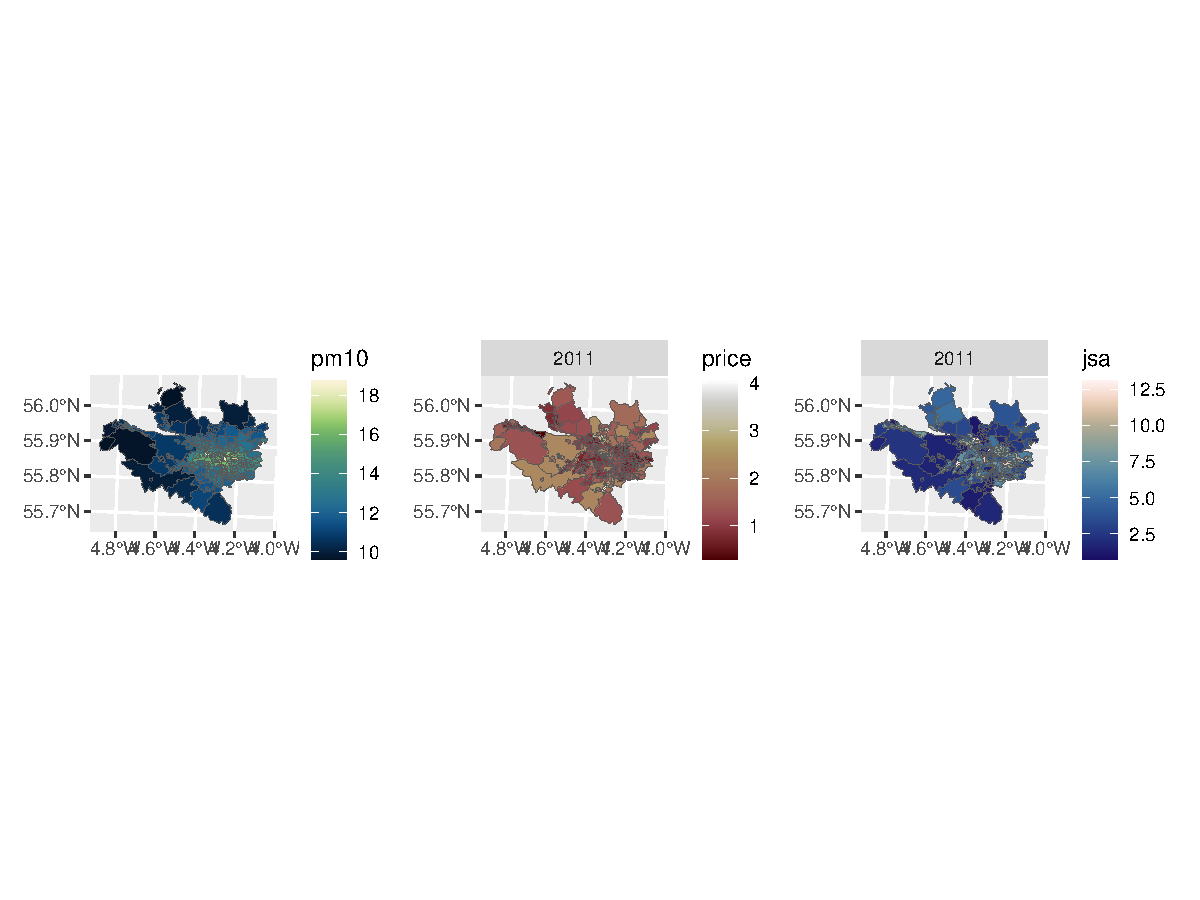
\includegraphics[keepaspectratio]{day2_practical_4_files/figure-pdf/unnamed-chunk-12-1.pdf}}
\end{center}

\end{tcolorbox}

As with the other types of spatial modelling, our goal is to observe and
explain spatial variation in our data. Generally, we are aiming to
produce a smoothed map which summarises the spatial patterns we observe
in our data.

A key aspect of any spatial analysis is that observations closer
together in space are likely to have more in common than those further
apart. This can lead us towards approaches similar to those used in time
series, where we consider the spatial \emph{closeness} of our regions in
terms of a \emph{neighbourhood structure}.

The function
\href{https://r-spatial.github.io/spdep/reference/poly2nb.html}{\texttt{poly2nb()}}
of the \texttt{spdep} package can be used to construct a list of
neighbors based on areas with contiguous boundaries (e.g., using Queen
contiguity).

\begin{Shaded}
\begin{Highlighting}[]
\FunctionTok{library}\NormalTok{(spdep)}

\NormalTok{W.nb }\OtherTok{\textless{}{-}} \FunctionTok{poly2nb}\NormalTok{(GGHB.IZ,}\AttributeTok{queen =} \ConstantTok{TRUE}\NormalTok{)}
\NormalTok{W.nb}
\end{Highlighting}
\end{Shaded}

\begin{verbatim}
Neighbour list object:
Number of regions: 271 
Number of nonzero links: 1424 
Percentage nonzero weights: 1.938971 
Average number of links: 5.254613 
2 disjoint connected subgraphs
\end{verbatim}

The warning tell us that the neighbourhood is comprised of two
interconnected regions. By looking at the neighbourhood graph below, we
can see that these are the North and South Glasgow regions which are
separated by the River Clyde.

\begin{Shaded}
\begin{Highlighting}[]
\FunctionTok{plot}\NormalTok{(}\FunctionTok{st\_geometry}\NormalTok{(GGHB.IZ), }\AttributeTok{border =} \StringTok{"lightgray"}\NormalTok{)}
\FunctionTok{plot.nb}\NormalTok{(W.nb, }\FunctionTok{st\_geometry}\NormalTok{(GGHB.IZ), }\AttributeTok{add =} \ConstantTok{TRUE}\NormalTok{)}
\end{Highlighting}
\end{Shaded}

\begin{center}
\pandocbounded{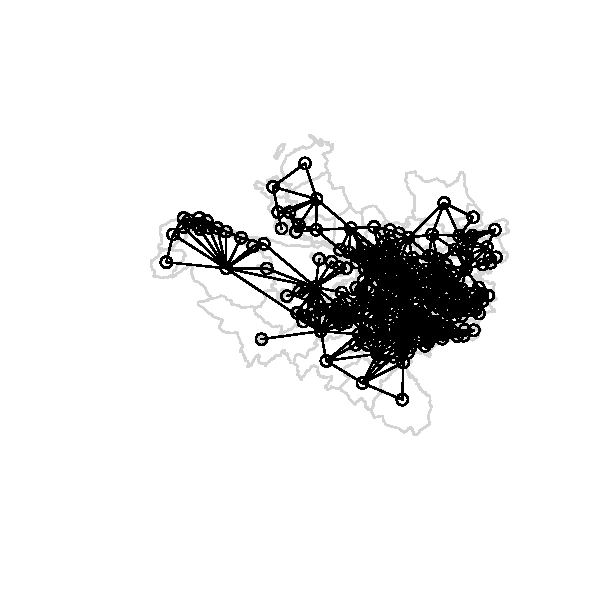
\includegraphics[keepaspectratio]{day2_practical_4_files/figure-pdf/unnamed-chunk-14-1.pdf}}
\end{center}

You could use the \texttt{snap} argument within \texttt{poly2nb} to set
a distance at which the different regions centroids are consider
neighbours. To do so we first need to be aware about the spatial units
of the spatial coordinate reference system (CRS). We can check this as
follows:

\begin{Shaded}
\begin{Highlighting}[]
\FunctionTok{st\_crs}\NormalTok{(GGHB.IZ)}\SpecialCharTok{$}\NormalTok{units}
\end{Highlighting}
\end{Shaded}

\begin{verbatim}
[1] "m"
\end{verbatim}

Then, we could set a distance of 250m to join the IZ centroids that are
are less than 250m apart.

\begin{Shaded}
\begin{Highlighting}[]
\NormalTok{W.nb250 }\OtherTok{\textless{}{-}} \FunctionTok{poly2nb}\NormalTok{(GGHB.IZ,}\AttributeTok{snap=}\DecValTok{250}\NormalTok{)}
\NormalTok{W.nb250}
\end{Highlighting}
\end{Shaded}

\begin{verbatim}
Neighbour list object:
Number of regions: 271 
Number of nonzero links: 1758 
Percentage nonzero weights: 2.393758 
Average number of links: 6.487085 
\end{verbatim}

\begin{Shaded}
\begin{Highlighting}[]
\FunctionTok{plot}\NormalTok{(}\FunctionTok{st\_geometry}\NormalTok{(GGHB.IZ), }\AttributeTok{border =} \StringTok{"lightgray"}\NormalTok{)}
\FunctionTok{plot.nb}\NormalTok{(W.nb250, }\FunctionTok{st\_geometry}\NormalTok{(GGHB.IZ), }\AttributeTok{add =} \ConstantTok{TRUE}\NormalTok{)}
\end{Highlighting}
\end{Shaded}

\begin{center}
\pandocbounded{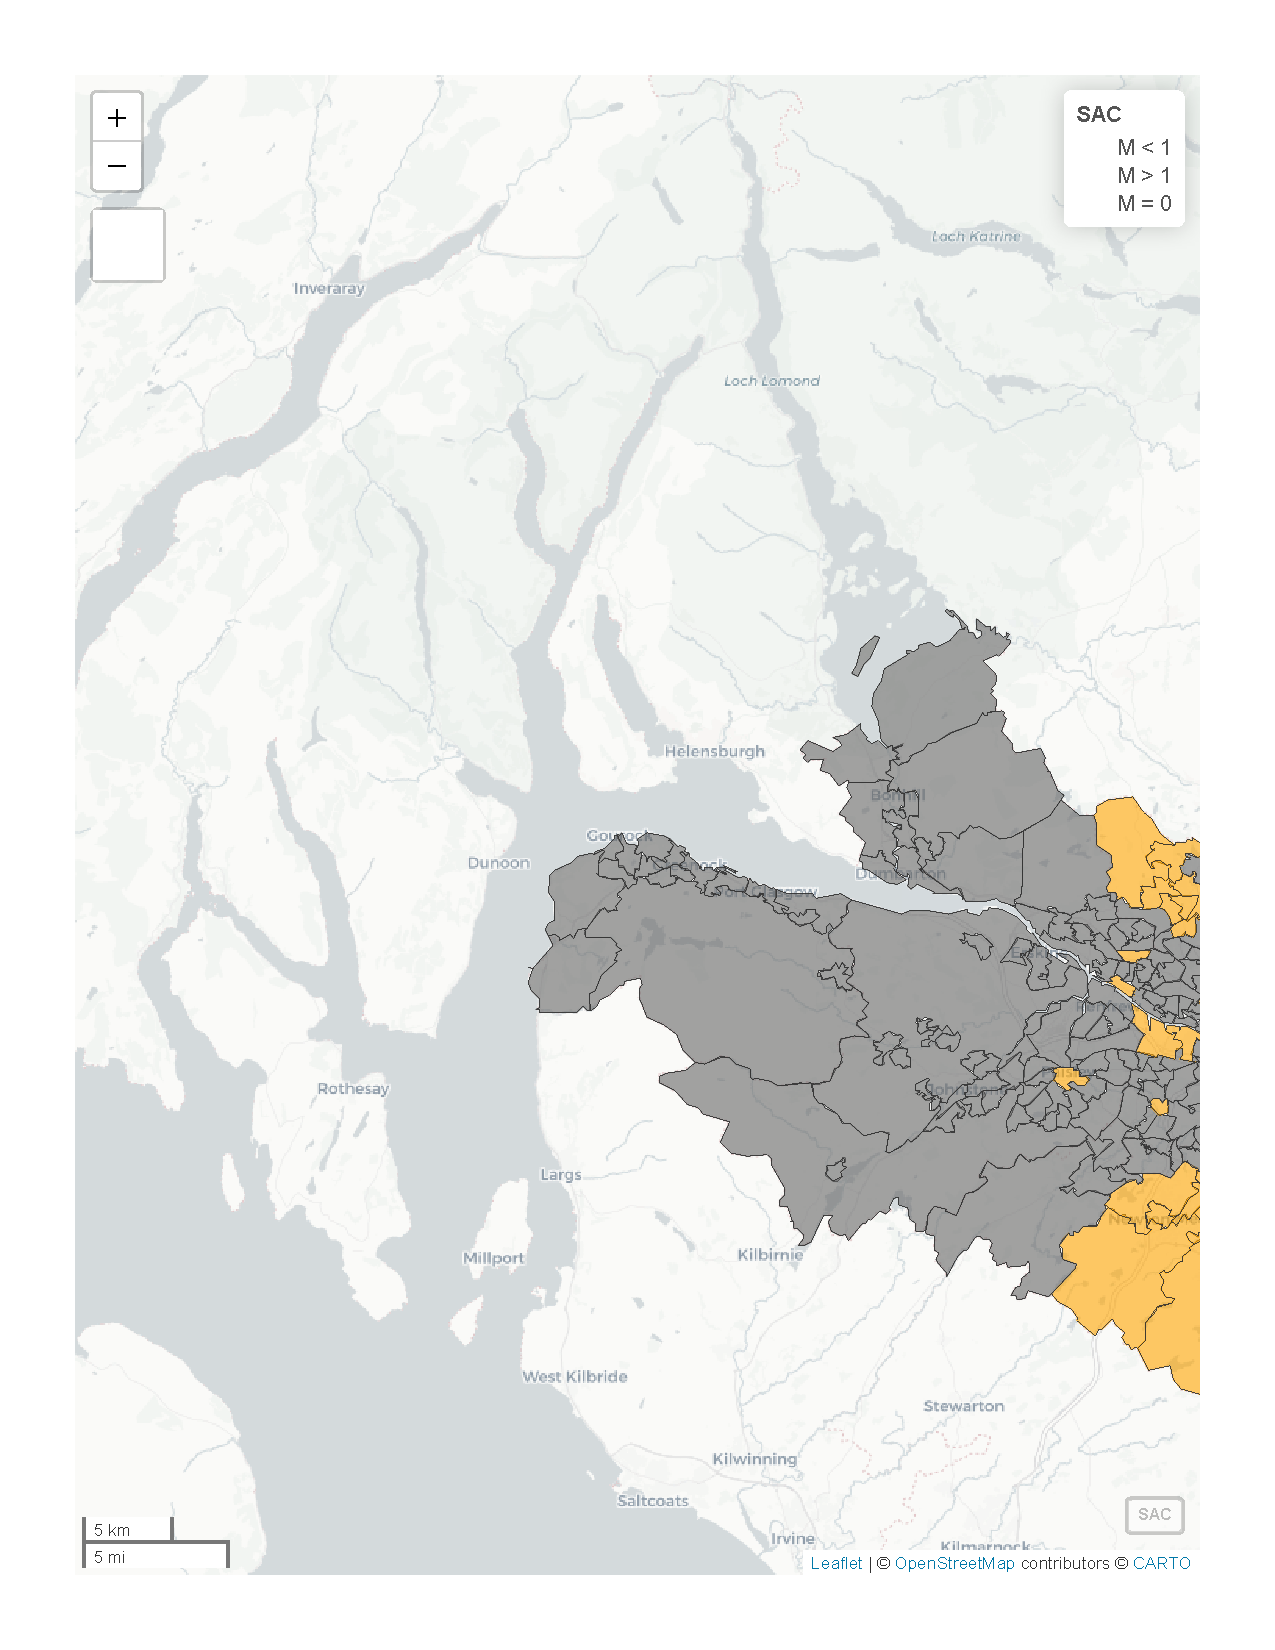
\includegraphics[keepaspectratio]{day2_practical_4_files/figure-pdf/unnamed-chunk-17-1.pdf}}
\end{center}

Once we have identified a set of neighbours using our chosen method, we
can use this to account for correlation.

Moran's \(I\) is a measure of global spatial autocorrelation, and can be
considered an extension of the Pearson correlation coefficient. For a
set of data \(Z_1, \ldots, Z_m\) measured on regions
\(B_1, \ldots B_m\), with neighbourhood matrix \(W\), we can compute
Moran's I as:

\[
I = \frac{m}{\sum_{i=1}^m \sum_{j=1}^m w_{ij}}\frac{\sum_{i=1}^m \sum_{j=1}^m w_{ij} (Z_i - \bar{Z})(Z_j - \bar{Z})}{\sum_{i=1}^m (Z_i - \bar{Z})^2}
\]

This is basically a function of differences in values between
neighbouring areas. By far the most common approach is to use a binary
neighbourhood matrix, \(W\), denoted by

\[ w_{ij} = \begin{cases} 1 & \text{if areas } (B_i, B_j) \text{ are neighbours.}\\ 0 & \text{otherwise.} \end{cases} \]

Binary matrices are used for their simplicity. Fitting spatial models
often requires us to invert \(W\), and this is less computationally
intensive for sparse matrices.

Moran's \(I\) ranges between -1 and 1, and can be interpreted in a
similar way to a standard correlation coefficient.

\begin{itemize}
\item
  \(I=1\) implies that we have \textbf{perfect spatial correlation}.
\item
  \(I=0\) implies that we have \textbf{complete spatial randomness}.
\item
  \(I=-1\) implies that we have \textbf{perfect dispersion} (negative
  correlation).
\end{itemize}

Our observed \(I\) is a point estimate, and we may also wish to assess
whether it is significantly different from zero. We can test for a
statistically significant spatial correlation using a permutation test,
with hypotheses:

\[
\begin{aligned}
H_0&: \text{ negative or no spatial association } (I \leq 0)\\
H_1&: \text{ positive spatial association } (I > 0)
\end{aligned}
\]

We can use \texttt{moran.test()} to test this hypothesis by setting
\texttt{alternative\ =\ "greater"}. To do so, we need to supply list
containing the neighbors via the \texttt{nb2listw()} function from the
\texttt{spdep} package. Lets assess now the spatial autocorrelation of
the SMR in 2011:

\begin{Shaded}
\begin{Highlighting}[]
\CommentTok{\# subset the data}
\NormalTok{resp\_cases\_2011 }\OtherTok{\textless{}{-}}\NormalTok{ resp\_cases }\SpecialCharTok{\%\textgreater{}\%} \FunctionTok{filter}\NormalTok{(year }\SpecialCharTok{==}\DecValTok{2011}\NormalTok{)}

\CommentTok{\# neighbors list }
\NormalTok{nbw }\OtherTok{\textless{}{-}} \FunctionTok{nb2listw}\NormalTok{(W.nb, }\AttributeTok{style =} \StringTok{"W"}\NormalTok{)}

\CommentTok{\# Global Moran\textquotesingle{}s I}
\NormalTok{gmoran }\OtherTok{\textless{}{-}} \FunctionTok{moran.test}\NormalTok{(resp\_cases\_2011}\SpecialCharTok{$}\NormalTok{SMR, nbw,}
                     \AttributeTok{alternative =} \StringTok{"greater"}\NormalTok{)}
\NormalTok{gmoran}
\end{Highlighting}
\end{Shaded}

\begin{verbatim}

    Moran I test under randomisation

data:  resp_cases_2011$SMR  
weights: nbw    

Moran I statistic standard deviate = 11.42, p-value < 2.2e-16
alternative hypothesis: greater
sample estimates:
Moran I statistic       Expectation          Variance 
      0.439899780      -0.003703704       0.001508809 
\end{verbatim}

\begin{tcolorbox}[enhanced jigsaw, bottomrule=.15mm, toprule=.15mm, rightrule=.15mm, arc=.35mm, coltitle=black, leftrule=.75mm, colframe=quarto-callout-tip-color-frame, colback=white, left=2mm, colbacktitle=quarto-callout-tip-color!10!white, bottomtitle=1mm, toptitle=1mm, titlerule=0mm, title={Question}, opacitybacktitle=0.6, opacityback=0, breakable]

What do we conclude from the Moran's I test?

Answer

Since have set the alternative hypothesis to be \$ I \textgreater{} 0 \$
and have a \emph{p}-value \(<0.05\), we then reject the null hypothesis
and conclude there is evidence for positive spatial autocorrelation.

\end{tcolorbox}

A local version of Moran's I can also be used to measure the similarity
between each IZ via the \texttt{localmoran} function:

\begin{Shaded}
\begin{Highlighting}[]
\NormalTok{lmoran }\OtherTok{\textless{}{-}} \FunctionTok{localmoran}\NormalTok{(resp\_cases\_2011}\SpecialCharTok{$}\NormalTok{SMR, nbw, }\AttributeTok{alternative =} \StringTok{"two.sided"}\NormalTok{)}
\end{Highlighting}
\end{Shaded}

In this case we set \texttt{alternative\ =\ "two.sided"} to test whether
there is any evidence of spatial autocorrelation in our data:

\[
\begin{aligned}
H_0&: \text{ no spatial association } (I=0)\\
H_1&: \text{ some spatial association } (I \neq 0)
\end{aligned}
\]

We can obtain the \(Z\)-scores from the test (\texttt{Z.Ii}) where any
values smaller than --1.96 indicate negative spatial autocorrelation,
and z-score values greater than 1.96 indicate positive spatial
autocorrelation:

\begin{Shaded}
\begin{Highlighting}[]
\NormalTok{resp\_cases\_2011\_m }\OtherTok{\textless{}{-}}\NormalTok{ resp\_cases\_2011 }\SpecialCharTok{\%\textgreater{}\%} \FunctionTok{mutate}\NormalTok{(}\AttributeTok{Zscores =}\NormalTok{ lmoran[,}\StringTok{"Z.Ii"}\NormalTok{])}

\NormalTok{resp\_cases\_2011\_m }\OtherTok{\textless{}{-}}\NormalTok{ resp\_cases\_2011\_m }\SpecialCharTok{\%\textgreater{}\%} 
  \FunctionTok{mutate}\NormalTok{ (}\AttributeTok{SAC =} \FunctionTok{case\_when}\NormalTok{(}
\NormalTok{  Zscores }\SpecialCharTok{\textgreater{}} \FunctionTok{qnorm}\NormalTok{(}\FloatTok{0.975}\NormalTok{) }\SpecialCharTok{\textasciitilde{}} \StringTok{" M \textgreater{} 1"}\NormalTok{ ,}
\NormalTok{  Zscores }\SpecialCharTok{\textless{}} \SpecialCharTok{{-}}\DecValTok{1}\SpecialCharTok{*}\FunctionTok{qnorm}\NormalTok{(}\FloatTok{0.975}\NormalTok{) }\SpecialCharTok{\textasciitilde{}} \StringTok{" M \textless{} 1"}\NormalTok{,}
  \AttributeTok{.default =} \StringTok{"M = 0"}\NormalTok{),}
  \AttributeTok{SAC=}\FunctionTok{as.factor}\NormalTok{(SAC)}
\NormalTok{)}
\end{Highlighting}
\end{Shaded}

We can visualize these results using either \texttt{ggplot} as we did
before, or via the \texttt{mapview} library which contains interactive
features:

\begin{Shaded}
\begin{Highlighting}[]
\FunctionTok{library}\NormalTok{(mapview)}
\FunctionTok{mapview}\NormalTok{(resp\_cases\_2011\_m, }
        \AttributeTok{zcol =} \StringTok{"SAC"}\NormalTok{,}
        \AttributeTok{layer.name =} \StringTok{"SAC"}\NormalTok{,}
        \AttributeTok{col.regions=}\FunctionTok{c}\NormalTok{(}\StringTok{"turquoise"}\NormalTok{,}\StringTok{"orange"}\NormalTok{,}\StringTok{"grey40"}\NormalTok{))}
\end{Highlighting}
\end{Shaded}

\begin{center}
\pandocbounded{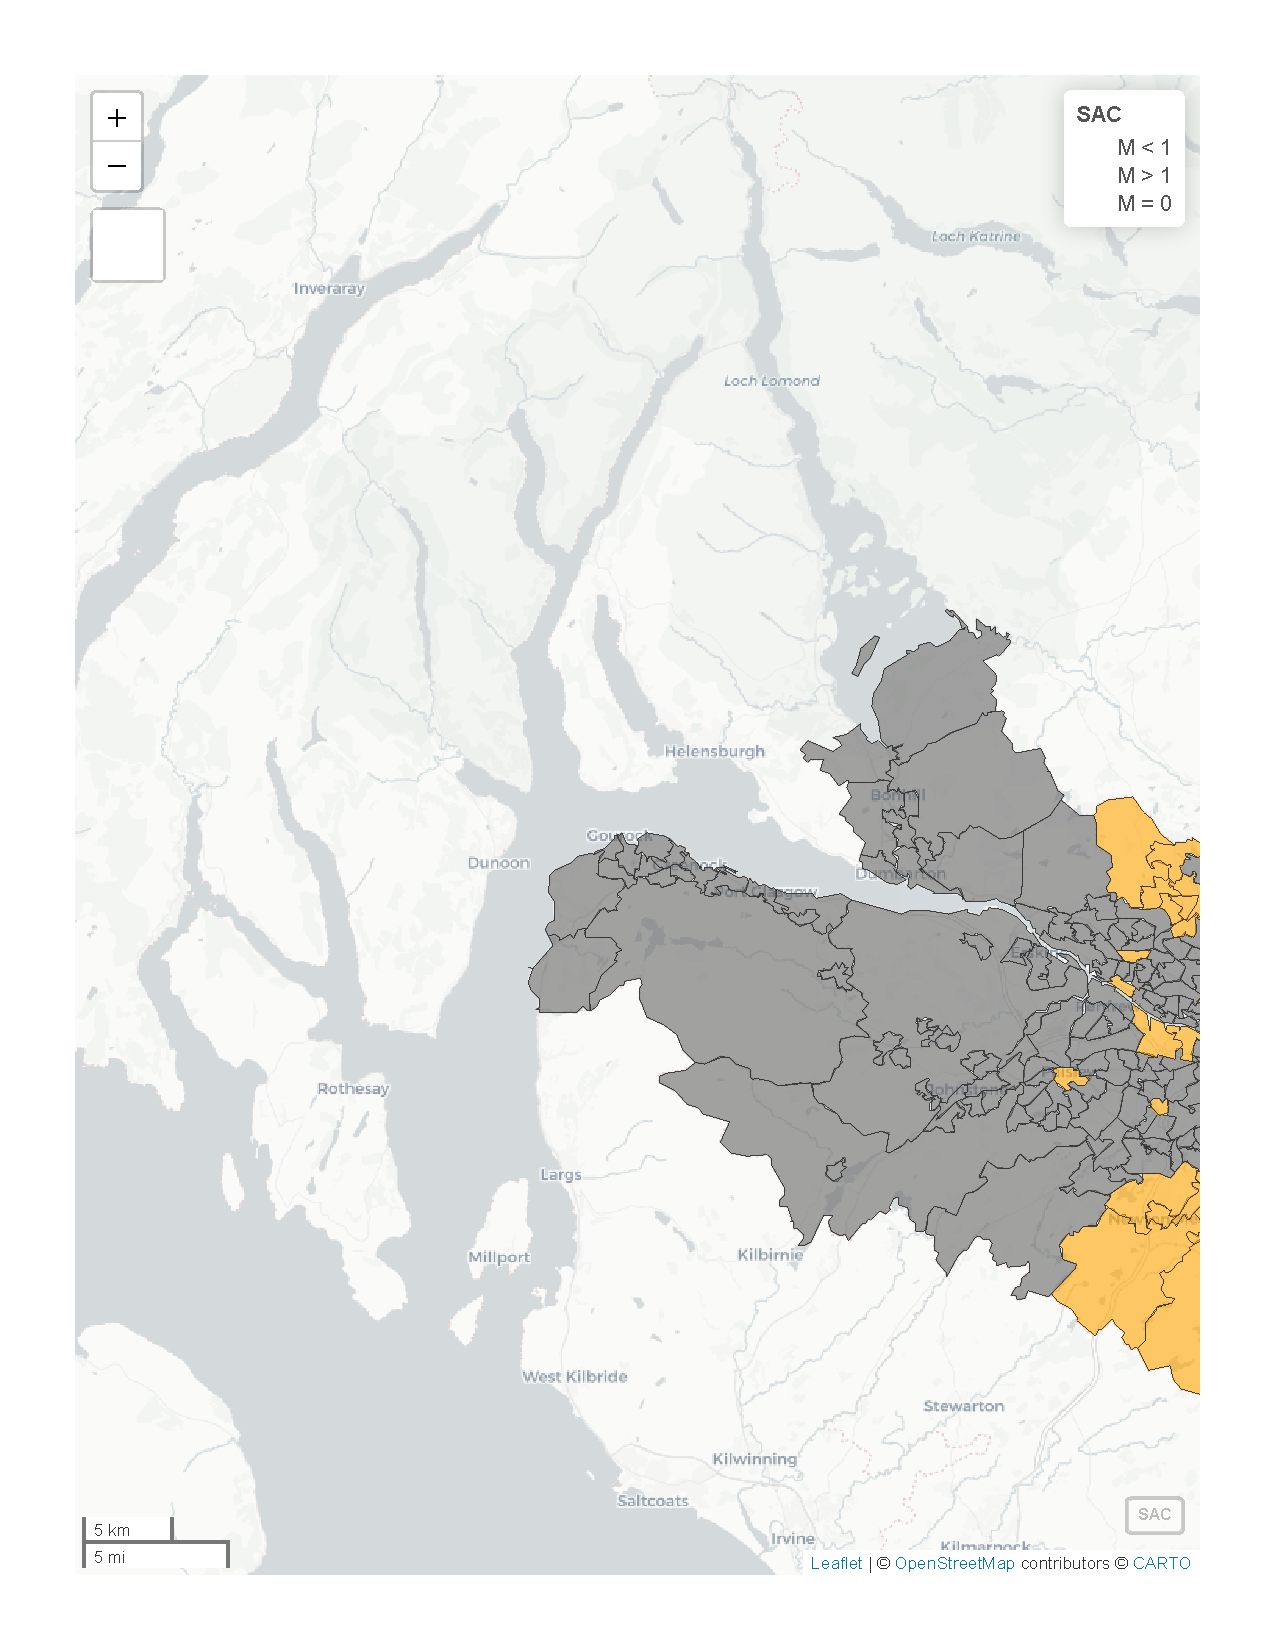
\includegraphics[keepaspectratio]{day2_practical_4_files/figure-pdf/unnamed-chunk-21-1.pdf}}
\end{center}

In this practical we will:

\begin{itemize}
\tightlist
\item
  Explore tools for geostatistical spatial data wrangling and
  visualization.
\item
  Compute a variogram to assess for spatial autocorrelation in our data.
\end{itemize}

First, lets load some useful libraries for data wrangling and
visualization

\begin{Shaded}
\begin{Highlighting}[]
\CommentTok{\# For plotting}
\FunctionTok{library}\NormalTok{(mapview)}
\FunctionTok{library}\NormalTok{(ggplot2)}
\FunctionTok{library}\NormalTok{(scico) }\CommentTok{\# for colouring palettes}

\CommentTok{\# Data manipulation}
\FunctionTok{library}\NormalTok{(dplyr)}
\end{Highlighting}
\end{Shaded}

\subsection{Geostatistical data}\label{geostatistical-data}

Tobler's first law of geography states that:

``\emph{Everything is related to everything else, but near things are
more related than distant things}''

Spatial patterns are fundamental in environmental and ecological data.
In many ecological and environmental settings, measurements from fixed
sampling units, aiming to quantify spatial variation and interpolate
values at unobserved sites.

\textbf{Geostatistical} data are the most common form of spatial data
found in environmental setting. In these data we regularly take
measurements of a spatial ecological or environmental process at a set
of fixed locations. This could be data from transects (e.g, where the
height of trees is recorded), samples taken across a region (e.g., water
depth in a lake) or from monitoring stations as part of a network (e.g.,
air pollution). In each of these cases, our goal is to estimate the
value of our variable across the entire space.

Let \(D\) be our two-dimensional region of interest. In principle, there
are infinite locations within \(D\), each of which can be represented by
mathematical coordinates (e.g., latitude and longitude). We then can
identify any individual location as \(s_i = (x_i, y_i)\), where \(x_i\)
and \(y_i\) are their coordinates.

We can treat our variable of interest as a random variable, \(Z\) which
can be observed at any location as \(Z(\mathbf{s}_i)\).

Our geostatistical process can therefore be written as:
\[\{Z(\mathbf{s}); \mathbf{s} \in D\}\]

In practice, our data are observed at a finite number of locations,
\(m\), and can be denoted as:

\[z = \{z(\mathbf{s}_1), \ldots z(\mathbf{s}_m) \}\]

In the next example, we will explore data on the Pacific Cod
(\emph{Gadus macrocephalus}) from a trawl survey in Queen Charlotte
Sound. The \texttt{pcod} dataset is available from the \texttt{sdmTMB}
package and contains the presence/absence records of the Pacific Cod
during each surveys along with the biomass density of Pacific cod in the
area swept (kg/Km\(^2\)). The \texttt{qcs\_grid} data contain the depth
values stored as \(2\times 2\) km grid for Queen Charlotte Sound.

\begin{Shaded}
\begin{Highlighting}[]
\FunctionTok{library}\NormalTok{(sdmTMB)}

\NormalTok{pcod\_df }\OtherTok{=}\NormalTok{ sdmTMB}\SpecialCharTok{::}\NormalTok{pcod }
\NormalTok{qcs\_grid }\OtherTok{=}\NormalTok{ sdmTMB}\SpecialCharTok{::}\NormalTok{qcs\_grid}
\end{Highlighting}
\end{Shaded}

\subsubsection{Georeferrenced data}\label{georeferrenced-data}

Let's create an initial \texttt{sf} spatial object using the standard
geographic coordinate system (\texttt{EPSG:4326}). This correctly
defines the point locations based on latitude and longitude.

\begin{Shaded}
\begin{Highlighting}[]
\FunctionTok{library}\NormalTok{(sf)}
\NormalTok{pcod\_sf }\OtherTok{=}   \FunctionTok{st\_as\_sf}\NormalTok{(pcod\_df, }\AttributeTok{coords =} \FunctionTok{c}\NormalTok{(}\StringTok{"lon"}\NormalTok{,}\StringTok{"lat"}\NormalTok{), }\AttributeTok{crs =} \DecValTok{4326}\NormalTok{)}
\end{Highlighting}
\end{Shaded}

Now we can transform to the standard UTM Zone 9N projection (EPSG:32609)
which uses meters:

\begin{Shaded}
\begin{Highlighting}[]
\NormalTok{pcod\_sf\_proj }\OtherTok{\textless{}{-}} \FunctionTok{st\_transform}\NormalTok{(pcod\_sf, }\AttributeTok{crs =} \DecValTok{32609}\NormalTok{)}
\FunctionTok{st\_crs}\NormalTok{(pcod\_sf\_proj)}\SpecialCharTok{$}\NormalTok{units}
\end{Highlighting}
\end{Shaded}

\begin{verbatim}
[1] "m"
\end{verbatim}

We can change the spatial units to \emph{km} to better reflect the scale
of our ecological study and to make resulting distance/area values more
intuitive to interpret:

\begin{Shaded}
\begin{Highlighting}[]
\NormalTok{pcod\_sf\_proj }\OtherTok{=} \FunctionTok{st\_transform}\NormalTok{(pcod\_sf\_proj,}
                            \FunctionTok{gsub}\NormalTok{(}\StringTok{"units=m"}\NormalTok{,}\StringTok{"units=km"}\NormalTok{,}
                                 \FunctionTok{st\_crs}\NormalTok{(pcod\_sf\_proj)}\SpecialCharTok{$}\NormalTok{proj4string)) }
\FunctionTok{st\_crs}\NormalTok{(pcod\_sf\_proj)}\SpecialCharTok{$}\NormalTok{units}
\end{Highlighting}
\end{Shaded}

\begin{verbatim}
[1] "km"
\end{verbatim}

Instead of first setting an EPSG code and then transforming, we can
define the target Coordinate Reference System (CRS) directly using a
\texttt{proj4string}. This allows us to customize non-standard
parameters in a single step, in this case, explicitly setting the
projection units to kilometers (\texttt{+units=km}).

\begin{Shaded}
\begin{Highlighting}[]
\NormalTok{pcod\_sf }\OtherTok{=} \FunctionTok{st\_transform}\NormalTok{(pcod\_sf,}
                       \AttributeTok{crs =} \StringTok{"+proj=utm +zone=9 +datum=WGS84 +no\_defs +type=crs +units=km"}\NormalTok{ )}
\FunctionTok{st\_crs}\NormalTok{(pcod\_sf)}\SpecialCharTok{$}\NormalTok{units}
\end{Highlighting}
\end{Shaded}

\begin{verbatim}
[1] "km"
\end{verbatim}

Spatial \texttt{sf} objects can be manipulated the same way we
manipulate standard data frame objects via the \texttt{dplyr} package.
For example, you can select a specific year using the \texttt{filter}
function from \texttt{dplyr}. Let's map the present/absence of the
Pacific Cod in 2017 using the \texttt{mapview} function:

\begin{Shaded}
\begin{Highlighting}[]
\NormalTok{pcod\_sf }\SpecialCharTok{\%\textgreater{}\%} 
  \FunctionTok{filter}\NormalTok{(year}\SpecialCharTok{==} \DecValTok{2017}\NormalTok{) }\SpecialCharTok{\%\textgreater{}\%}
  \FunctionTok{mutate}\NormalTok{(}\AttributeTok{present =} \FunctionTok{as.factor}\NormalTok{(present)) }\SpecialCharTok{\%\textgreater{}\%}
\FunctionTok{mapview}\NormalTok{(}\AttributeTok{zcol =} \StringTok{"present"}\NormalTok{,}
        \AttributeTok{layer.name =} \StringTok{"Occupancy status of Pacific Code in 2017"}\NormalTok{)}
\end{Highlighting}
\end{Shaded}

\begin{center}
\pandocbounded{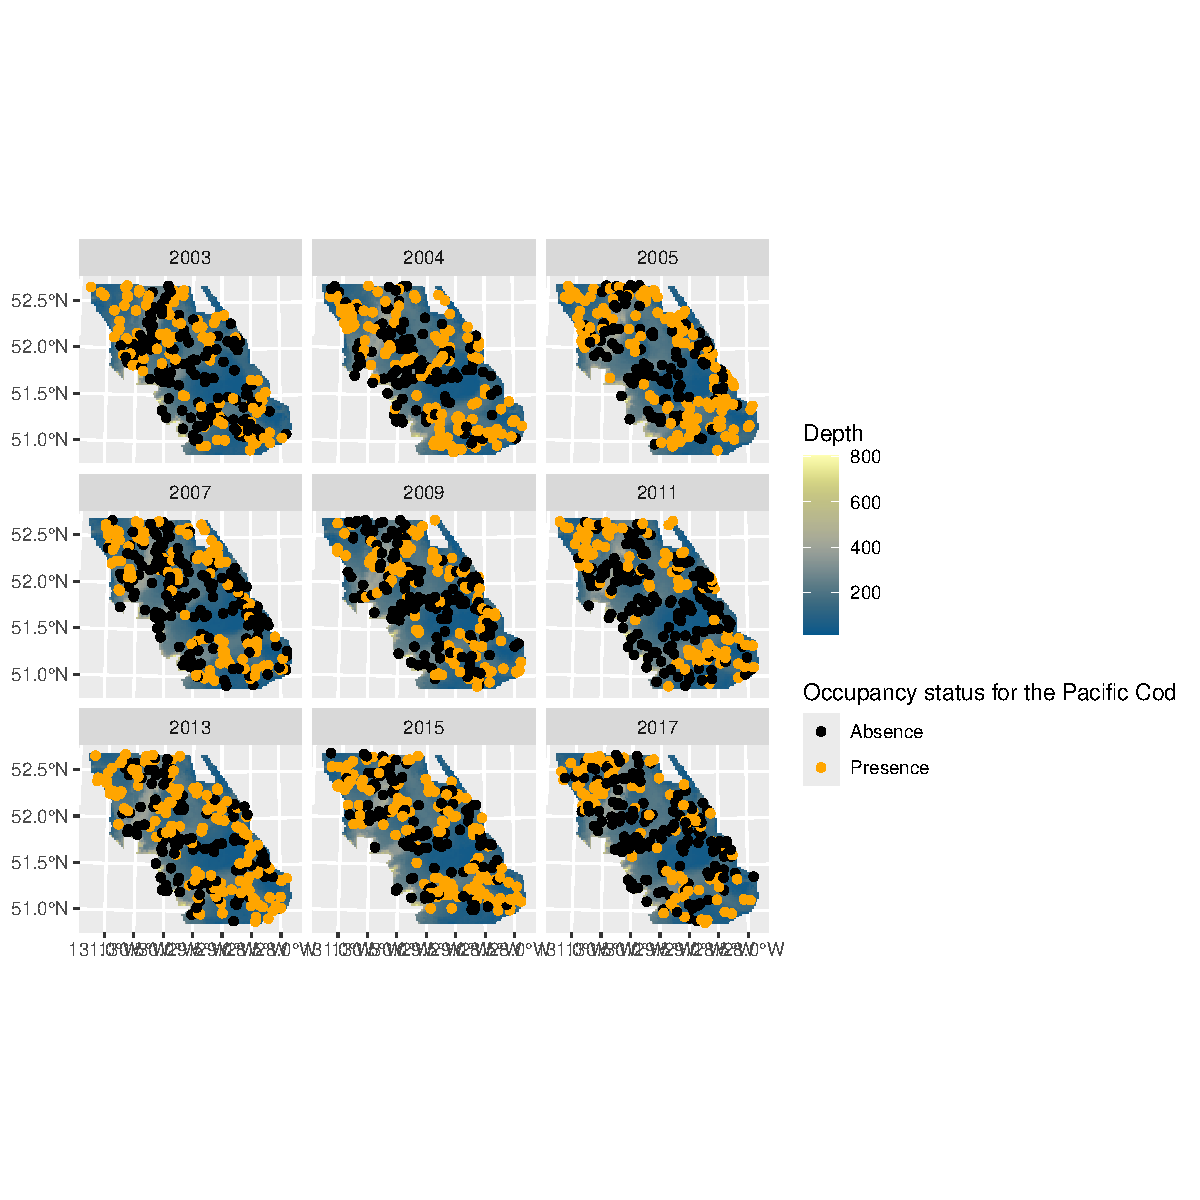
\includegraphics[keepaspectratio]{day2_practical_4_files/figure-pdf/unnamed-chunk-47-1.pdf}}
\end{center}

\begin{tcolorbox}[enhanced jigsaw, bottomrule=.15mm, toprule=.15mm, rightrule=.15mm, arc=.35mm, coltitle=black, leftrule=.75mm, colframe=quarto-callout-warning-color-frame, colback=white, left=2mm, colbacktitle=quarto-callout-warning-color!10!white, bottomtitle=1mm, toptitle=1mm, titlerule=0mm, title={Task}, opacitybacktitle=0.6, opacityback=0, breakable]

Use \texttt{ggplot} and the \texttt{sf} library to map the biomass
density of the pacific code across years.

hint

You can plot an\texttt{sf} object by adding a \texttt{geom\_sf} layer to
a ggplot object. You can also use the \texttt{facet\_wrap} argument to
plot an arrange of plots according to a grouping variable.

Click here to see the solution

\begin{Shaded}
\begin{Highlighting}[]
\FunctionTok{ggplot}\NormalTok{()}\SpecialCharTok{+} 
  \FunctionTok{geom\_sf}\NormalTok{(}\AttributeTok{data=}\NormalTok{pcod\_sf,}\FunctionTok{aes}\NormalTok{(}\AttributeTok{color=}\NormalTok{density))}\SpecialCharTok{+} 
  \FunctionTok{facet\_wrap}\NormalTok{(}\SpecialCharTok{\textasciitilde{}}\NormalTok{year)}\SpecialCharTok{+}
  \FunctionTok{theme}\NormalTok{(}\AttributeTok{legend.position =} \StringTok{"bottom"}\NormalTok{)}
\end{Highlighting}
\end{Shaded}

\begin{center}
\pandocbounded{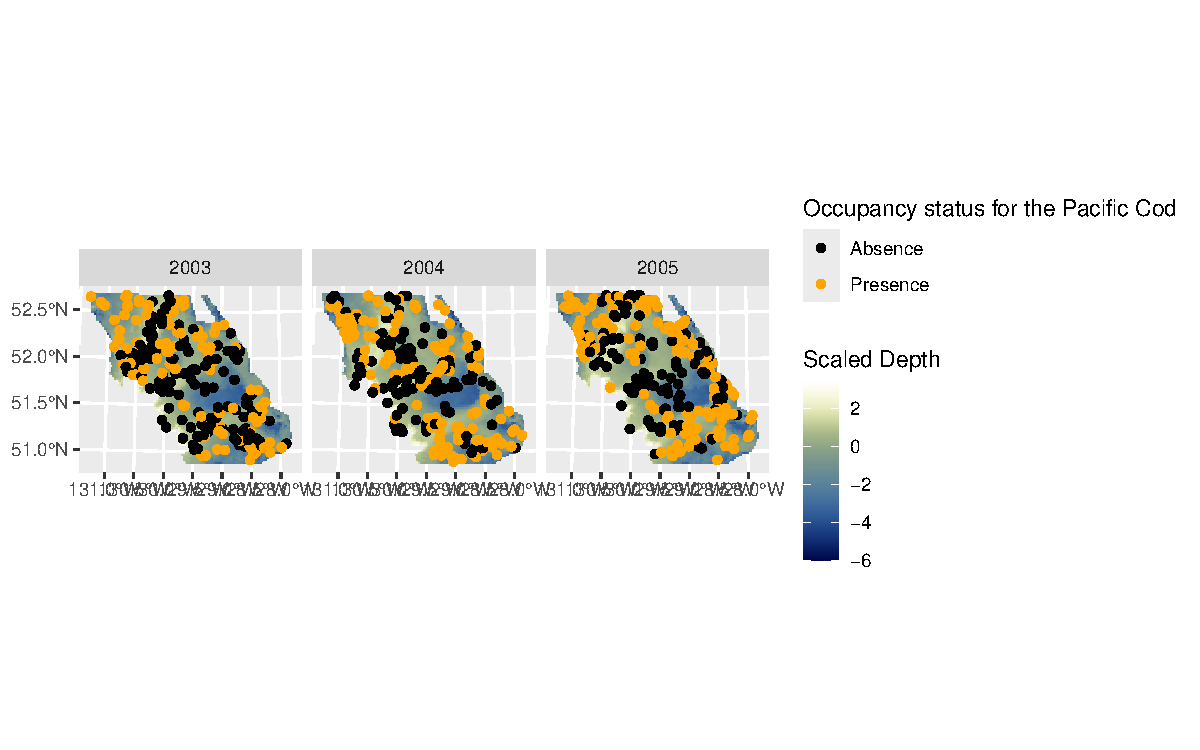
\includegraphics[keepaspectratio]{day2_practical_4_files/figure-pdf/unnamed-chunk-48-1.pdf}}
\end{center}

\end{tcolorbox}

\subsubsection{Raster Data}\label{raster-data}

Environmental data is typically stored in raster format, which
represents spatially continuous phenomena by dividing a region into a
grid of equally-sized cells, each storing a value for the variable of
interest. In R, the \texttt{terra} package is a modern and powerful tool
for efficiently working with raster data. The function \texttt{rast()},
can be used both to read raster files from standard formats (e.g.,
\texttt{.tif} or \texttt{.tiff}) and to create a new raster object from
a data frame. For instance, the following code creates a raster from the
\texttt{qcs\_grid} grid data for Queen Charlotte Sound.

\begin{Shaded}
\begin{Highlighting}[]
\FunctionTok{library}\NormalTok{(terra)}
\NormalTok{depth\_r }\OtherTok{\textless{}{-}} \FunctionTok{rast}\NormalTok{(qcs\_grid, }\AttributeTok{type =} \StringTok{"xyz"}\NormalTok{)}
\NormalTok{depth\_r}
\end{Highlighting}
\end{Shaded}

\begin{verbatim}
class       : SpatRaster 
size        : 102, 121, 3  (nrow, ncol, nlyr)
resolution  : 2, 2  (x, y)
extent      : 341, 583, 5635, 5839  (xmin, xmax, ymin, ymax)
coord. ref. :  
source(s)   : memory
names       :    depth, depth_scaled, depth_scaled2 
min values  :  12.0120,    -6.000040,  4.892624e-08 
max values  : 805.7514,     3.453937,  3.600048e+01 
\end{verbatim}

The raster object contains three layers corresponding to the (i) depth
values, (ii) the scaled depth values and (iii) the squared depth values.

Notice that there are no CRS associated with the raster. Thus, we can
assign appropriate CRS using the \texttt{crs} function. Additionally, we
also want the raster CRS to match the CRS in the survey data (recall
that we have previously reprojected our data to utm coordinates). We can
assign an appropiate CRS that matches the CRS of the \texttt{sf} object
as follows:

\begin{Shaded}
\begin{Highlighting}[]
\FunctionTok{crs}\NormalTok{(depth\_r) }\OtherTok{\textless{}{-}} \FunctionTok{crs}\NormalTok{(pcod\_sf)}
\end{Highlighting}
\end{Shaded}

We can use the \texttt{tidyterra} package to plot raster data using
\texttt{ggplot} by adding a \texttt{geom\_spatraster} function and then
select an appropriate \texttt{fill} and \texttt{color} palettes:

\begin{Shaded}
\begin{Highlighting}[]
\FunctionTok{library}\NormalTok{(tidyterra)}
\end{Highlighting}
\end{Shaded}

\begin{verbatim}

Attaching package: 'tidyterra'
\end{verbatim}

\begin{verbatim}
The following object is masked from 'package:stats':

    filter
\end{verbatim}

\begin{Shaded}
\begin{Highlighting}[]
\FunctionTok{ggplot}\NormalTok{()}\SpecialCharTok{+} 
  \FunctionTok{geom\_spatraster}\NormalTok{(}\AttributeTok{data=}\NormalTok{depth\_r}\SpecialCharTok{$}\NormalTok{depth)}\SpecialCharTok{+}
  \FunctionTok{geom\_sf}\NormalTok{(}\AttributeTok{data=}\NormalTok{pcod\_sf,}\FunctionTok{aes}\NormalTok{(}\AttributeTok{color=}\FunctionTok{factor}\NormalTok{(present))) }\SpecialCharTok{+}
  \FunctionTok{facet\_wrap}\NormalTok{(}\SpecialCharTok{\textasciitilde{}}\NormalTok{year)}\SpecialCharTok{+}
    \FunctionTok{scale\_color\_manual}\NormalTok{(}\AttributeTok{name=}\StringTok{"Occupancy status for the Pacific Cod"}\NormalTok{,}
                     \AttributeTok{values =} \FunctionTok{c}\NormalTok{(}\StringTok{"black"}\NormalTok{,}\StringTok{"orange"}\NormalTok{),}
                     \AttributeTok{labels=} \FunctionTok{c}\NormalTok{(}\StringTok{"Absence"}\NormalTok{,}\StringTok{"Presence"}\NormalTok{))}\SpecialCharTok{+}
  \FunctionTok{scale\_fill\_scico}\NormalTok{(}\AttributeTok{name =} \StringTok{"Depth"}\NormalTok{,}
                   \AttributeTok{palette =} \StringTok{"nuuk"}\NormalTok{,}
                   \AttributeTok{na.value =} \StringTok{"transparent"}\NormalTok{ )}
\end{Highlighting}
\end{Shaded}

\begin{center}
\pandocbounded{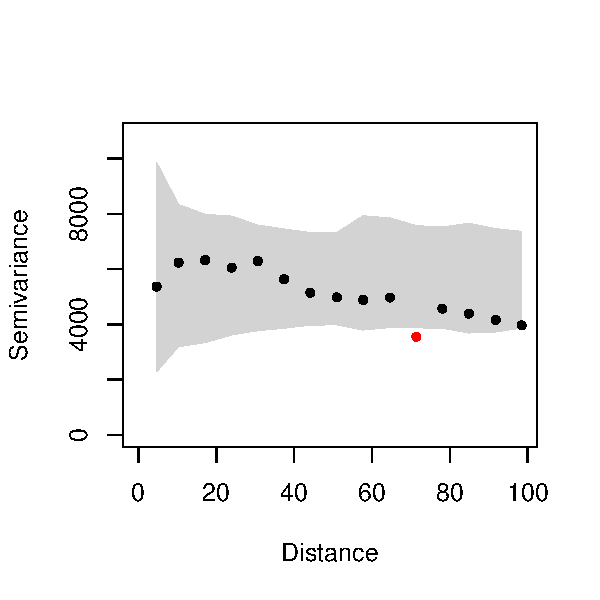
\includegraphics[keepaspectratio]{day2_practical_4_files/figure-pdf/unnamed-chunk-51-1.pdf}}
\end{center}

\begin{tcolorbox}[enhanced jigsaw, bottomrule=.15mm, toprule=.15mm, rightrule=.15mm, arc=.35mm, coltitle=black, leftrule=.75mm, colframe=quarto-callout-warning-color-frame, colback=white, left=2mm, colbacktitle=quarto-callout-warning-color!10!white, bottomtitle=1mm, toptitle=1mm, titlerule=0mm, title={Task}, opacitybacktitle=0.6, opacityback=0, breakable]

Map the scaled depth and the presence/absence records of the Pacific cod
for 2003 to 2005 only.

hint

The different layers of a raster can be accessed using the \texttt{\$}
symbol.

Click here to see the solution

\begin{Shaded}
\begin{Highlighting}[]
\FunctionTok{ggplot}\NormalTok{()}\SpecialCharTok{+} 
  \FunctionTok{geom\_spatraster}\NormalTok{(}\AttributeTok{data=}\NormalTok{depth\_r}\SpecialCharTok{$}\NormalTok{depth\_scaled)}\SpecialCharTok{+}
  \FunctionTok{geom\_sf}\NormalTok{(}\AttributeTok{data=}\NormalTok{pcod\_sf }\SpecialCharTok{\%\textgreater{}\%} \FunctionTok{filter}\NormalTok{(year }\SpecialCharTok{\%in\%} \DecValTok{2003}\SpecialCharTok{:}\DecValTok{2005}\NormalTok{),}
          \FunctionTok{aes}\NormalTok{(}\AttributeTok{color=}\FunctionTok{factor}\NormalTok{(present)))}\SpecialCharTok{+} 
  \FunctionTok{facet\_wrap}\NormalTok{(}\SpecialCharTok{\textasciitilde{}}\NormalTok{year)}\SpecialCharTok{+}
  \FunctionTok{scale\_color\_manual}\NormalTok{(}\AttributeTok{name=}\StringTok{"Occupancy status for the Pacific Cod"}\NormalTok{,}
                     \AttributeTok{values =} \FunctionTok{c}\NormalTok{(}\StringTok{"black"}\NormalTok{,}\StringTok{"orange"}\NormalTok{),}
                     \AttributeTok{labels=} \FunctionTok{c}\NormalTok{(}\StringTok{"Absence"}\NormalTok{,}\StringTok{"Presence"}\NormalTok{))}\SpecialCharTok{+}
    \FunctionTok{scale\_fill\_scico}\NormalTok{(}\AttributeTok{name =} \StringTok{"Scaled Depth"}\NormalTok{,}
                     \AttributeTok{palette =} \StringTok{"davos"}\NormalTok{,}
                     \AttributeTok{na.value =} \StringTok{"transparent"}\NormalTok{ )}
\end{Highlighting}
\end{Shaded}

\begin{center}
\pandocbounded{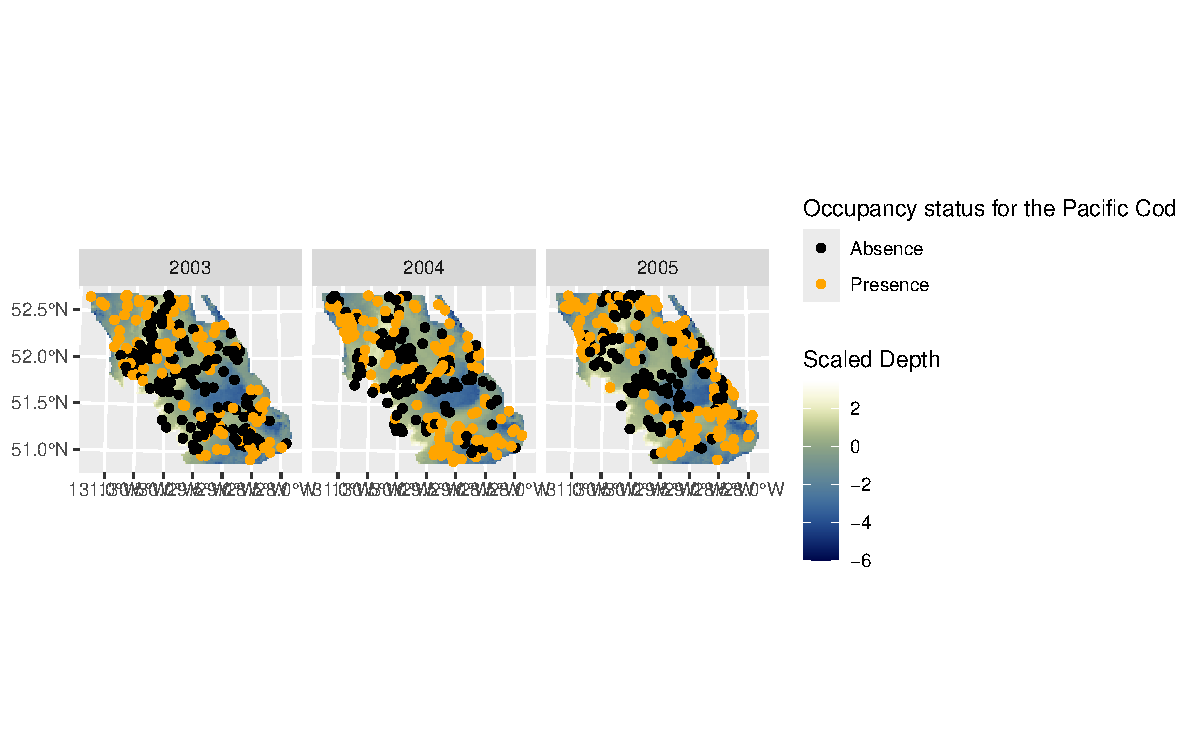
\includegraphics[keepaspectratio]{day2_practical_4_files/figure-pdf/unnamed-chunk-52-1.pdf}}
\end{center}

\end{tcolorbox}

\subsubsection{Autocorrelation and
Variograms}\label{autocorrelation-and-variograms}

Spatial statistics quantifies the fundamental principle that nearby
things are more related. This spatial dependence means that data points
are not independent, as assumed by most classical statistical models,
but are instead correlated based on their proximity. While this
correlation can be a valuable source of information, it must be
explicitly accounted for to avoid biased inference and incorrect
conclusions.

The first step is to assess whether there is any evidence of spatial
dependency in our data. Spatial dependence can be explored by a function
known as a variogram \(2\gamma(\cdot)\) (or semivariogram
\(\gamma(\cdot)\)). The variogram is similar in many ways to the
autocorrelation function used in time series modelling. In simple terms,
it is a function which measures the difference in the spatial process
between a pair of locations a fixed distance apart

The variogram measures the variance of the difference in the process
\(Z(\cdot)\) at two spatial locations \(\mathbf{s}\) and
\(\mathbf{s+h}\) and is defined as :

\[\mathrm{Var}[Z(\mathbf{s}) - Z(\mathbf{s} + \mathbf{h})] = E[(Z(\mathbf{s}) - Z(\mathbf{s} + \mathbf{h}))^2] = 2\gamma_z(\mathbf{h}).\]

Here, \(2\gamma_z(\mathbf{h})\) is the variogram, but in practice we use
the semi-variogram, \(\gamma_z(\mathbf{h})\). We use the semi-variogram
because our points come in pairs, and the semi-variance is equivalent to
the variance per point at a given lag.

\begin{itemize}
\item
  When the variance of the difference \(Z(\mathbf{s}) - Z(\mathbf{t})\)
  is relatively small, then \(Z(\mathbf{s})\) and \(Z(\mathbf{t})\) are
  similar (spatially correlated).
\item
  When the variance of the difference \(Z(\mathbf{s}) - Z(\mathbf{t})\)
  is relatively large, then \(Z(\mathbf{s})\) and \(Z(\mathbf{t})\) are
  less similar (closer to independence).
\end{itemize}

The variogram is a function of the underlying geostatistical process
\(Z\). In practice, we only have access to \(m\) realisations of this
process, and therefore we have to estimate the variogram. This is known
as the empirical variogram.

We obtain this by computing the semi-variance for all possible pairs of
observations:
\(\gamma(\mathbf{s}, \mathbf{t}) = 0.5(Z(\mathbf{s}) - Z(\mathbf{t}))^2\).

\begin{tcolorbox}[enhanced jigsaw, bottomrule=.15mm, toprule=.15mm, rightrule=.15mm, arc=.35mm, coltitle=black, leftrule=.75mm, colframe=quarto-callout-note-color-frame, colback=white, left=2mm, colbacktitle=quarto-callout-note-color!10!white, bottomtitle=1mm, toptitle=1mm, titlerule=0mm, title={Example}, opacitybacktitle=0.6, opacityback=0, breakable]

To illustrate how an empirical variogram is computed, consider the
biomass density of the Pacific Cod in 2017 for the two highlighted
locations below.

\begin{center}
\pandocbounded{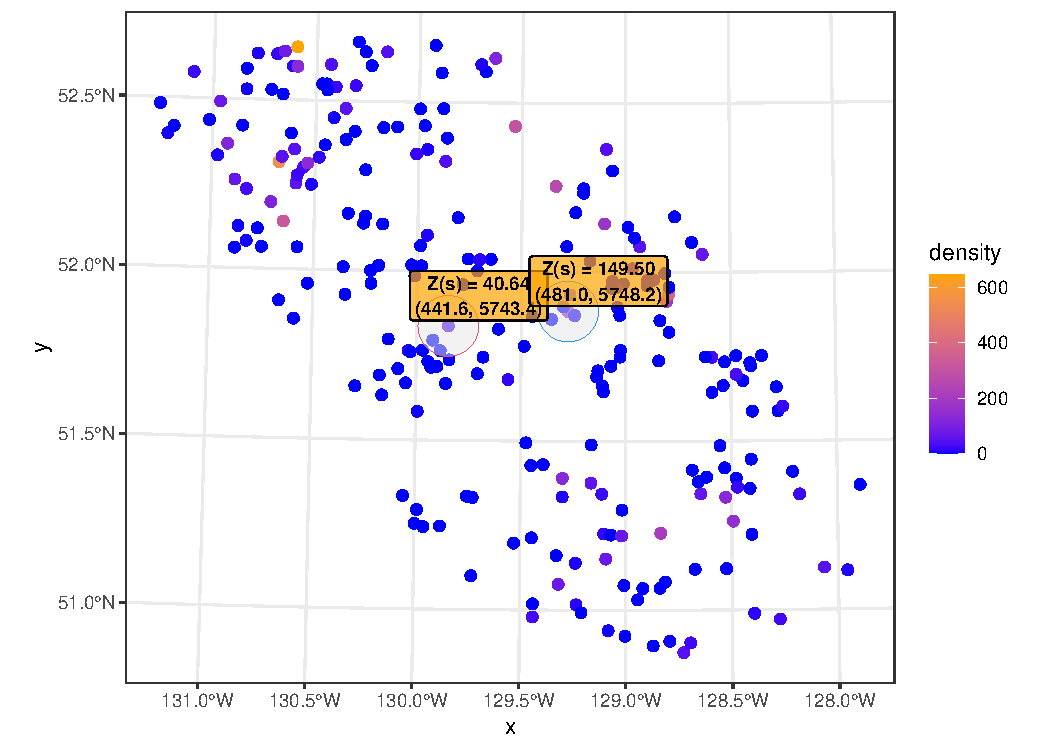
\includegraphics[keepaspectratio]{day2_practical_4_files/figure-pdf/unnamed-chunk-53-1.pdf}}
\end{center}

\begin{enumerate}
\def\labelenumi{\arabic{enumi}.}
\tightlist
\item
  We can first compute the distance between the two locations using the
  standard Euclidean distance formula as
\end{enumerate}

\[h = \sqrt{(441.6 -481)^2 + (5743.4-5748.2)^2} \approx  39 ~\text{Km}\]

\begin{enumerate}
\def\labelenumi{\arabic{enumi}.}
\setcounter{enumi}{1}
\item
  Next, we compute the semi-variance between the points using their
  observed values as
  \[\gamma(\mathbf{s}, \mathbf{t}) = 0.5(Z(\mathbf{s}) - Z(\mathbf{t}))^2 = 0.5(149.5 - 40.64)^2 = 5925.25\]
\item
  We repeat this process for every possible pair of points, and plot
  \(h\) against \(\gamma(\mathbf{s}, \mathbf{t})\) for each.
\end{enumerate}

\end{tcolorbox}

To make the variogram easier to use and interpret, we divide the
distances into a set of discrete bins, and compute the average
semi-variance in each. We compute this binned empirical variogram as:

\[\gamma(\mathbf{h}) = \frac{1}{2N(h_k)}\sum_{(\mathbf{s},\mathbf{t}) \in N(h_k)}[z(\mathbf{s}) - z(\mathbf{t})]^2\]

We can calculate the binned- empirical variogram for the data using
\texttt{variogram} function from the \texttt{gstat} library. This plot
shows the semi-variances for each pair of points. Lets compute a
variogram for the biomass density of the Pacific Cod in 2017:

\begin{Shaded}
\begin{Highlighting}[]
\FunctionTok{library}\NormalTok{(gstat)}

\NormalTok{pcod\_sf\_subset }\OtherTok{\textless{}{-}}\NormalTok{ pcod\_sf }\SpecialCharTok{\%\textgreater{}\%} \FunctionTok{filter}\NormalTok{(year }\SpecialCharTok{==}\DecValTok{2017}\NormalTok{)}

\NormalTok{vgm1 }\OtherTok{\textless{}{-}} \FunctionTok{variogram}\NormalTok{(density}\SpecialCharTok{\textasciitilde{}}\DecValTok{1}\NormalTok{, pcod\_sf\_subset)}
\FunctionTok{plot}\NormalTok{(vgm1)}
\end{Highlighting}
\end{Shaded}

\begin{center}
\pandocbounded{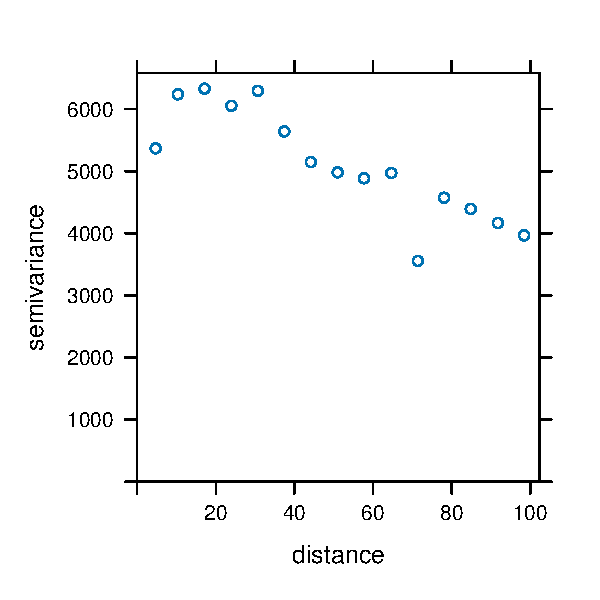
\includegraphics[keepaspectratio]{day2_practical_4_files/figure-pdf/unnamed-chunk-54-1.pdf}}
\end{center}

\textbf{Assessing spatial dependence}

We can construct null envelope based on permutations of the data values
across the locations, i.e.~envelopes built under the assumption of no
spatial correlation. By overlapping these envelopes with the empirical
variograms we can determine whether there is some spatial dependence in
our data ,e.g.~if our observed variograms falls outside of the envelopes
constructed under spatial randomness.

We can construct permutation envelopes on the gstat empirical variogram
using the \texttt{envelope} function from the \texttt{variosig} R
package. Then we can visualize the results using the \texttt{envplot}
function:

\begin{Shaded}
\begin{Highlighting}[]
\FunctionTok{library}\NormalTok{(variosig)}

\NormalTok{varioEnv }\OtherTok{\textless{}{-}} \FunctionTok{envelope}\NormalTok{(vgm1,}
                     \AttributeTok{data =}\NormalTok{ pcod\_sf\_subset,}
                     \AttributeTok{locations =} \FunctionTok{st\_coordinates}\NormalTok{(pcod\_sf\_subset),}
                     \AttributeTok{formula =}\NormalTok{ density }\SpecialCharTok{\textasciitilde{}} \DecValTok{1}\NormalTok{,}
                     \AttributeTok{nsim =} \DecValTok{499}\NormalTok{)}

\FunctionTok{envplot}\NormalTok{(varioEnv)}
\end{Highlighting}
\end{Shaded}

\begin{center}
\pandocbounded{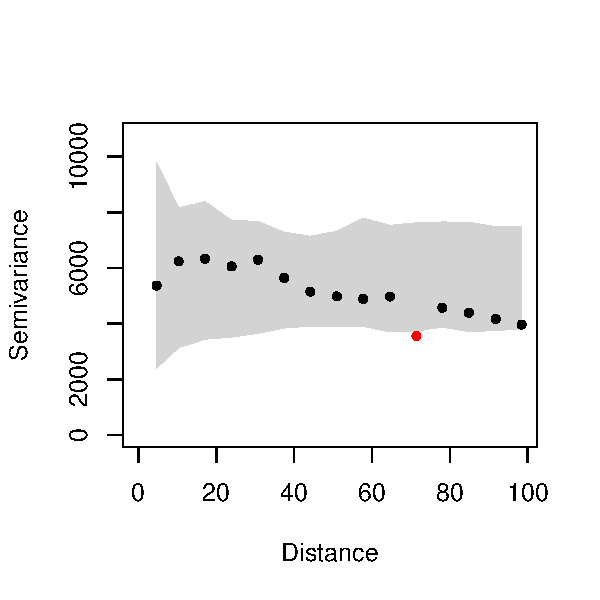
\includegraphics[keepaspectratio]{day2_practical_4_files/figure-pdf/unnamed-chunk-55-1.pdf}}
\end{center}

\begin{verbatim}
[1] "There are 1 out of 15 variogram estimates outside the 95% envelope."
\end{verbatim}




\end{document}
